\documentclass{article}


\usepackage{arxiv}

\usepackage[utf8]{inputenc} % allow utf-8 input
\usepackage[T1]{fontenc}    % use 8-bit T1 fonts
\usepackage{hyperref}       % hyperlinks
\usepackage{url}            % simple URL typesetting
\usepackage{booktabs}       % professional-quality tables
\usepackage{amsfonts}       % blackboard math symbols
\usepackage{nicefrac}       % compact symbols for 1/2, etc.
\usepackage{microtype}      % microtypography
\usepackage{multirow}
\usepackage{multicol}
\usepackage{graphicx}
%\usepackage{natbib}
\usepackage[numbers,sort&compress]{natbib}
\usepackage{hyperref}
\usepackage{amsmath}
\usepackage{amssymb}
\usepackage{mathtools, nccmath}
%\usepackage{subcaption}
\usepackage{float}
\DeclarePairedDelimiter{\nint}\lfloor\rceil
\usepackage[linesnumbered,ruled,vlined]{algorithm2e}
%%%%%%%%%%% Defining Enunciations  %%%%%%%%%%%
\newtheorem{theorem}{\bf Theorem}[section]
\newtheorem{condition}{\bf Condition}[section]
\newtheorem{corollary}{\bf Corollary}[section]
%%%%%%%%%%%%%%%%%%%%%%%%%%%%%%%%%%%%%%%%%%%%%%%


\title{Dealing with uncertainty in agent-based models for short-term predictions}


\author{
  Le-Minh Kieu\thanks{Corresponding author} \\
  School of Geography \& Leeds Institute of Data Analytics\\
  University of Leeds\\
  United Kingdom \\
  \texttt{m.l.kieu@leeds.ac.uk} \\
  %% examples of more authors
   \And
 Nicolas Malleson \\
  School of Geography\\
  University of Leeds and Alan Turing Institute\\
  United Kingdom \\
  \texttt{n.s.malleson@leeds.ac.uk} \\
  \And
 Alison Heppenstall \\
  School of Geography\\
  University of Leeds and Alan Turing Institute\\
  United Kingdom \\
  \texttt{a.j.heppenstall@leeds.ac.uk} \\
}

\begin{document}
\maketitle

\begin{abstract}
Agent-based models (ABM) are gaining traction as one of the most powerful modelling tools within the social sciences.
They are particularly suited to simulating complex systems. Despite many methodological advances within ABM, one of the major drawbacks is their inability to 
incorporate real-time data to make accurate short-term predictions. This paper presents an approach that allows ABMs to be dynamically optimised. Through a combination of parameter calibration and data assimilation (DA), the accuracy of model-based predictions using ABM in real time is increased.  We use the exemplar of a bus route system to explore these methods.  
%Within this paper we construct an ABM that simulates the main interactions and key processes within this system. We develop an numerical experiment to quantify the impacts of calibration and DA in dealing the with stochastic and dynamic nature of the system under study. 
The bus route ABMs developed in this research are examples of ABMs that can be dynamically optimised by a combination of parameter calibration and DA. The proposed model and framework can also be used in an passenger information system, or in an Intelligent Transport Systems to provide forecasts of bus locations and arrival times. 
\end{abstract}


% keywords can be removed
\keywords{First keyword \and Second keyword \and More}


\section{Introduction} 
\label{s:Intro}

Agent-based modelling (ABM) \citep{bonabeau_agent_2002} is a field that excels in its ability to simulate
complex systems. Instead of deriving aggregated equations of system
dynamics, ABM encapsulates system-wide characteristics from the
behaviours and interactions of individual agents e.g. human, animals
or vehicles. ABM has emerged as an important tool for many 
applications ranging from urban traffic simulation
\citep{balmer2009matsim}, humanitarian assistance
\citep{crooks_gis_2013} to emergency evacuations
\citep{schoenharl_design_2011}.

Despite the many advances and applications of ABM, the field suffers from a serious drawback: models are currently  unable to incorporate up-to-date data to make accurate real-time predictions \citep{lloyd_exploring_2016, wang_data_2015,
ward_dynamic_2016}. Models are typically calibrated once, using historical data, then projected forward in time to make a prediction. Here, calibration is ideal for one point in time, but as the simulation progresses, the prediction rapidly diverges from reality  due to underlying uncertainties \citep{ward_dynamic_2016}. These uncertainties come from \textit{dynamic} (changing over space and time), \textit{stochastic} (containing inherent randomness) and \textit{unobserved} (unseen from the data) conditions of the real system under study. An example of such a system can be found in bus routes. Each time a bus reaches a bus stop, the number of alighting passengers is uncertain and the number of waiting passengers downstream is unobserved. The bus route's conditions also change over time, e.g. traffic varies over the route and with at off-peak to peak periods. 
%\end{fmtext}
There are methods to incorporate streaming data into models,
such as \textit{data assimilation} (DA) routines
\citep{lewis_dynamic_2006, wang2000data}. Broadly, DA refers to a suite of techniques that allow
observational data to be incorporated into models
\citep{wang2000data} to provide an optimal estimate of the
evolving state of the system. Performing DA increases the
probability of having an accurate representation of the current state of
the system, thereby reducing the uncertainty of future predictions. This is a technique that has been widely applied
in fields such as meteorology, hydrology and oceanography \citep{kalnay_atmospheric_2003}.

There are, however, two methodological challenges that must be overcome to apply DA in ABM. First, DA methods are often intrinsic to their underlying models which are typically systems of partial differential equations with functions linearised mathematically.  Hence DA methods typically rely on linearising the underlying model \citep{harvey1990forecasting}. One of the most appealing aspects of agent-based models is that they are inherently non-linear, so it is not clear whether the assumptions of traditional DA methods will hold. Second, it is still unknown how much uncertainty DA can effectively deal with when implemented within ABM. Assimilation of real-time data into ABMs has only been attempted a few times and these examples are limited by their simplicity \citep{lloyd_exploring_2016, wang_data_2015,
ward_dynamic_2016}.

This paper is part of a wider programme of work\footnote{\url{http://dust.leeds.ac.uk/}} that is focused on developing DA methods to be readily used in ABM. This paper focuses on one particular model that aims  to make predictions of bus locations in real time. Bus route operation has been chosen due to its inherent uncertainties -- for example a model will need to account for uncertain factors affecting how buses travel on the roads \citep{khosravi2011prediction} -- but also for its tractability -- there are many fewer interactions than present in, say, a model of a crowd.  We also focus on one particular DA algorithm -- the Particle Filter (PF). This method is chosen due to its ability to incorporate data into non-linear models such as ABMs \citep{carpenter1999improved}.

The objectives of this paper are to: (1) perform dynamic state estimation to reduce the
uncertainty in the model's estimate of the \textit{current} system state; (2) improve the accuracy of short term forecasts.

All the numerical experiments in this paper will be tightly controlled, following an `identical twin' experimental framework \citep[for example see][]{wang_data_2015}. We will first develop a complex ABM of a bus route to generate fine-grained synthetic GPS data of buses, that are reasonably similar to real GPS data, for use as synthetic `ground truth' data. We call this model the `BusSim-truth' model. The next step
is to develop companion ABMs that are of simpler nature than BusSim-truth that will not know the parameters of BusSim-truth and will not have the dynamic and stochastic features of BusSim-truth. We will calibrate and evaluate these companion ABMs against the data generated from BusSim-truth. This experiment is designed to be similar to the real-time monitoring and predictions of bus locations, where models are often a simpler version of reality, that are calibrated to be as close as possible to reality. The prediction of bus location and arrival times are essential for bus operators and a topical research challenge \citep{bin2006bus}. The methods developed here can easily be applied to simulation and forecasting for \textit{real} bus systems and could, therefore, offer considerable potential impact. This is particularly pertinent in rapidly developing cities where daily bus schedules can be extremely erratic. In these cases accurate, up-to-date estimates of current waiting times will be highly beneficial to citizens who use (or would like to use) public transport. 

The contributions of this paper are threefold. First, several ABMs of bus routes are constructed that account for the interactions between the bus and passengers, the bus and the surrounding traffic, and between multiple buses are considered. While model development is not the sole focus of this paper, these bus route ABMs are novel and have utility for other studies. Second, this paper introduces a combination of parameter calibration and DA techniques that can dynamically optimise an ABM to enable accurate estimation of the bus system in real time. Third, this paper shows and quantifies the impacts of calibration and DA in dealing the with stochastic and dynamic nature of the system under study.

This paper is structured as follows. Section~\ref{s:problem} describes
the research problem and the related works in the literature.
Section~\ref{s:method} outlines the methodology. Section~\ref{s:experiments} describes
the numerical experiments that are conducted and discusses these
results. Finally, Section~\ref{s:conclusion} concludes the study and
considers the opportunities for future work. 

% Other sections are in their own file

% !TEX root = BusSim.tex
% 
\section{Research problem and related works} \label{s:problem}

Historical and real-time bus GPS data is often used by operators to locate buses and predict their locations and arrival times. For instance, Public Transport Information and Priority System (PTIPS) is a state-of-the-art system in Australia to give priority to public transport vehicles on the roads and provide information on predicted bus arrival to passengers. The prediction of bus locations and arrival times in real time is a challenging problem \citep{chien2002dynamic}. Ideally, perfect 
knowledge of the current state of the system and any underlying processes is required.  However, obtaining this level of knowledge is impossible due to sources of uncertainty and the complex interactions in
bus operations. The majority of research within this area has focused on machine learning methods to find a direct mapping between input
data and bus arrival time. Examples of these methods include Artificial
Neural Networks \citep{chien2002dynamic}, Support Vector Machines
\citep{bin2006bus}, and Bayesian techniques
\citep{khosravi2011prediction}. While machine learning methods are generally
efficient in real time, they are solely reliant on the quality of available
data. Even with high-resolution datasets that record accurate spatio-temporal bus locations, the full complexity of the system will never be captured. 

%Without an understanding of the underlying processes driving bus operation, these models fail to quantify uncertainty and will perform poorly in highly stochastic systems, in unseen situations or when data are missing.

There are analytical and simulation models of bus routes that aim to
reproduce the underlying processes in bus operations, and shed some
light on the associated uncertainties. One of the earliest successes in simulating a simple bus systems was from Cellular Automata modelling
\citep{luo2012realistic,o1998jamming,chowdhury2000steady,
jiang2003realistic}. Whilst the dynamical foundations of these models
are well understood, they are outperformed by more sophisticated
models such as bus-following models
\citep{nagatani2000kinetic,huijberts2002analysis,Tang2012,
nagatani2001bunching,hill2003numerical}; and traffic-following models
\citep{cats2010mesoscopic,toledo2010mesoscopic,hans2015real}.
Bus-following models aim to model the fundamental dynamics of a bus
route by modelling individual buses that follow each other (for example speeding up if the bus ahead is far away). Traffic-following models,
on the other hand, aim to model buses as a component of a transport
system with private and public transport, where their speeds are
affected by the traffic flow, traffic signals \citep{hans2015real} or
traffic density \citep{toledo2010mesoscopic}.

The majority of these models are \textit{static}, i.e. they only have parameters that are fixed over time. We can represent these static simulators 
with the equation $Y = f(X)$, where $f$ represents the simulator. A run of a simulation is defined
as the process of producing one set of data $Y$ for a single set of
model parameters $X$. One way for these
models to reduce their uncertainty and fit more closely to the observed data is to
adjust the model parameters until the model satisfies some predetermined
criteria. This parameter adjustment process is often referred to as
\textit{parameter calibration}. Popular optimisation techniques include simulated annealing~\citep{pennisi_optimal_2008}, genetic
algorithms,~\citep{heppenstall_genetic_2007, malleson_optimising_2014},
and approximate Bayesian computation~\citep{grazzini_bayesian_2017}.
Parameter calibration, especially with ABMs, is often only
implemented once, and therefore cannot account for any changes that may take place within
the system. In the traffic context these might include accidents, traffic signal failures, vehicle faults, etc. Static models are simple to implement, but struggle to model dynamic systems. 


%Many advanced simulators are now \textit{dynamic}: they have inputs and
%outputs that vary over time and operate iteratively over fixed
%time steps. A real bus route is an example of a dynamic system, where
%the arrival rate of passengers and the surrounding traffic vary across
%different times of day, days of the week, and even seasonally. A dynamic
%simulator may be written in the form $Y_t = f(X_t)$, where $Y_t$ is the
%set of outputs at time $t$ and $X_t$ subsumes both fixed model
%parameters and time-varying variables at time step $t$. 

In real-time applications, e.g bus location or bus arrival time prediction in real time, prediction models often have to deal with the fact that there are so much uncertainty in bus operations. Real bus operation is \textit{dynamic} (changing over time) and also \textit{stochastic} (contains inherent randomness). In real time, there are also many unobservable information of bus operation, such as the number of passengers who are waiting at
downstream stops or the number who plan to get off the bus, and the
surrounding traffic conditions.  The lack of information about these factors means that any model of bus
operation in real time will have to make assumptions thereby introducing uncertainties. 

Therefore, this research will explore a combination of parameter calibration and a \textit{data
assimilation} (DA) technique to calibrate a dynamic ABM bus route simulator using historical data, and then dynamically optimised it on-the-fly using real-time data. This, in itself, is a novel and important
contribution. Few previous efforts have attempted to incorporate data
assimilation with agent-based models \citep[for example
see][]{ward_dynamic_2016, wang_data_2015}, and it is unclear how DA
methods, that have typically been created for linear models
\citep{harvey1990forecasting}, can be adapted for non-linear ABMs. 

DA methods assume that observational data are sparse and only describe
the target system in limited detail. Therefore a model is essential as a
means of filling in the gaps in space and time left by the observations through the generation of additional data.
In effect, the model propagates data from observed to unobserved areas
\citep{carrassi_data_2018}.  Although techniques can be used to
perform parameter estimation, they are most often framed as a state
estimation problem. The aim is to calculate a posterior probability for
the state vector $X_t$, given prior distributions from a model (in this
case, a bus route operation model) and data from observations. It is
this marriage of a model and real-time observational data (and the 
associated uncertainties) that offers the means of allowing all the
available information to be used to determine the true state of the
system as accurately as possible \citep{talagrand_use_1991}.

Models where the system state at time $t$ are only dependent on the state at time $t-1$ are termed \textit{Markovian}. We are particularly interested in ABMs that can be written in a Markovian nature because DA algorithms require knowledge to the \textit{full} model state in the form of the state vector $X_t$. While some ABMs in the literature track agent histories and use this information to decide future states, these can be recast as Markovian ABMs by expanding the state vector to include these histories. Implementing a bus route system as a Markovian model requires variables such as vehicle locations, speeds, occupancies etc. It is reasonable to
assume that the system state at the next time step only depends on the
value of these variables at the current time step. For simplicity, we
assume that the state vector used here has a fixed size.  The unused variables (i.e. those for buses that have yet to enter the system) can be set to zero, enabling the state vector to be treated as sparse and
passed efficiently between iterations. If the state vector has a fixed
size, then all possible states of the system belongs to a state-space
$\mathcal{X} \in \mathbb{R}^n$. The system state evolves in some fixed
interval \{0,..,K\}. We denote the state of the bus route at time $t$ by
$X_t \in \mathcal{X}$.

This paper follows an `identical twin' experiment framework \cite{wang_data_2015}, where experiment data to be used will be generated from simulation, instead of using real data. The reason is that real data often comes with noise that hides the true state of the bus route (e.g. noise from GPS data). A simulated synthetic data would enable us to control the level of noise in the data, and to evaluate the modelling results against the ground truth rather than noisy data. Figure \ref{fig:workflow} shows the workflow of this study. 

\begin{figure}[H]  \centering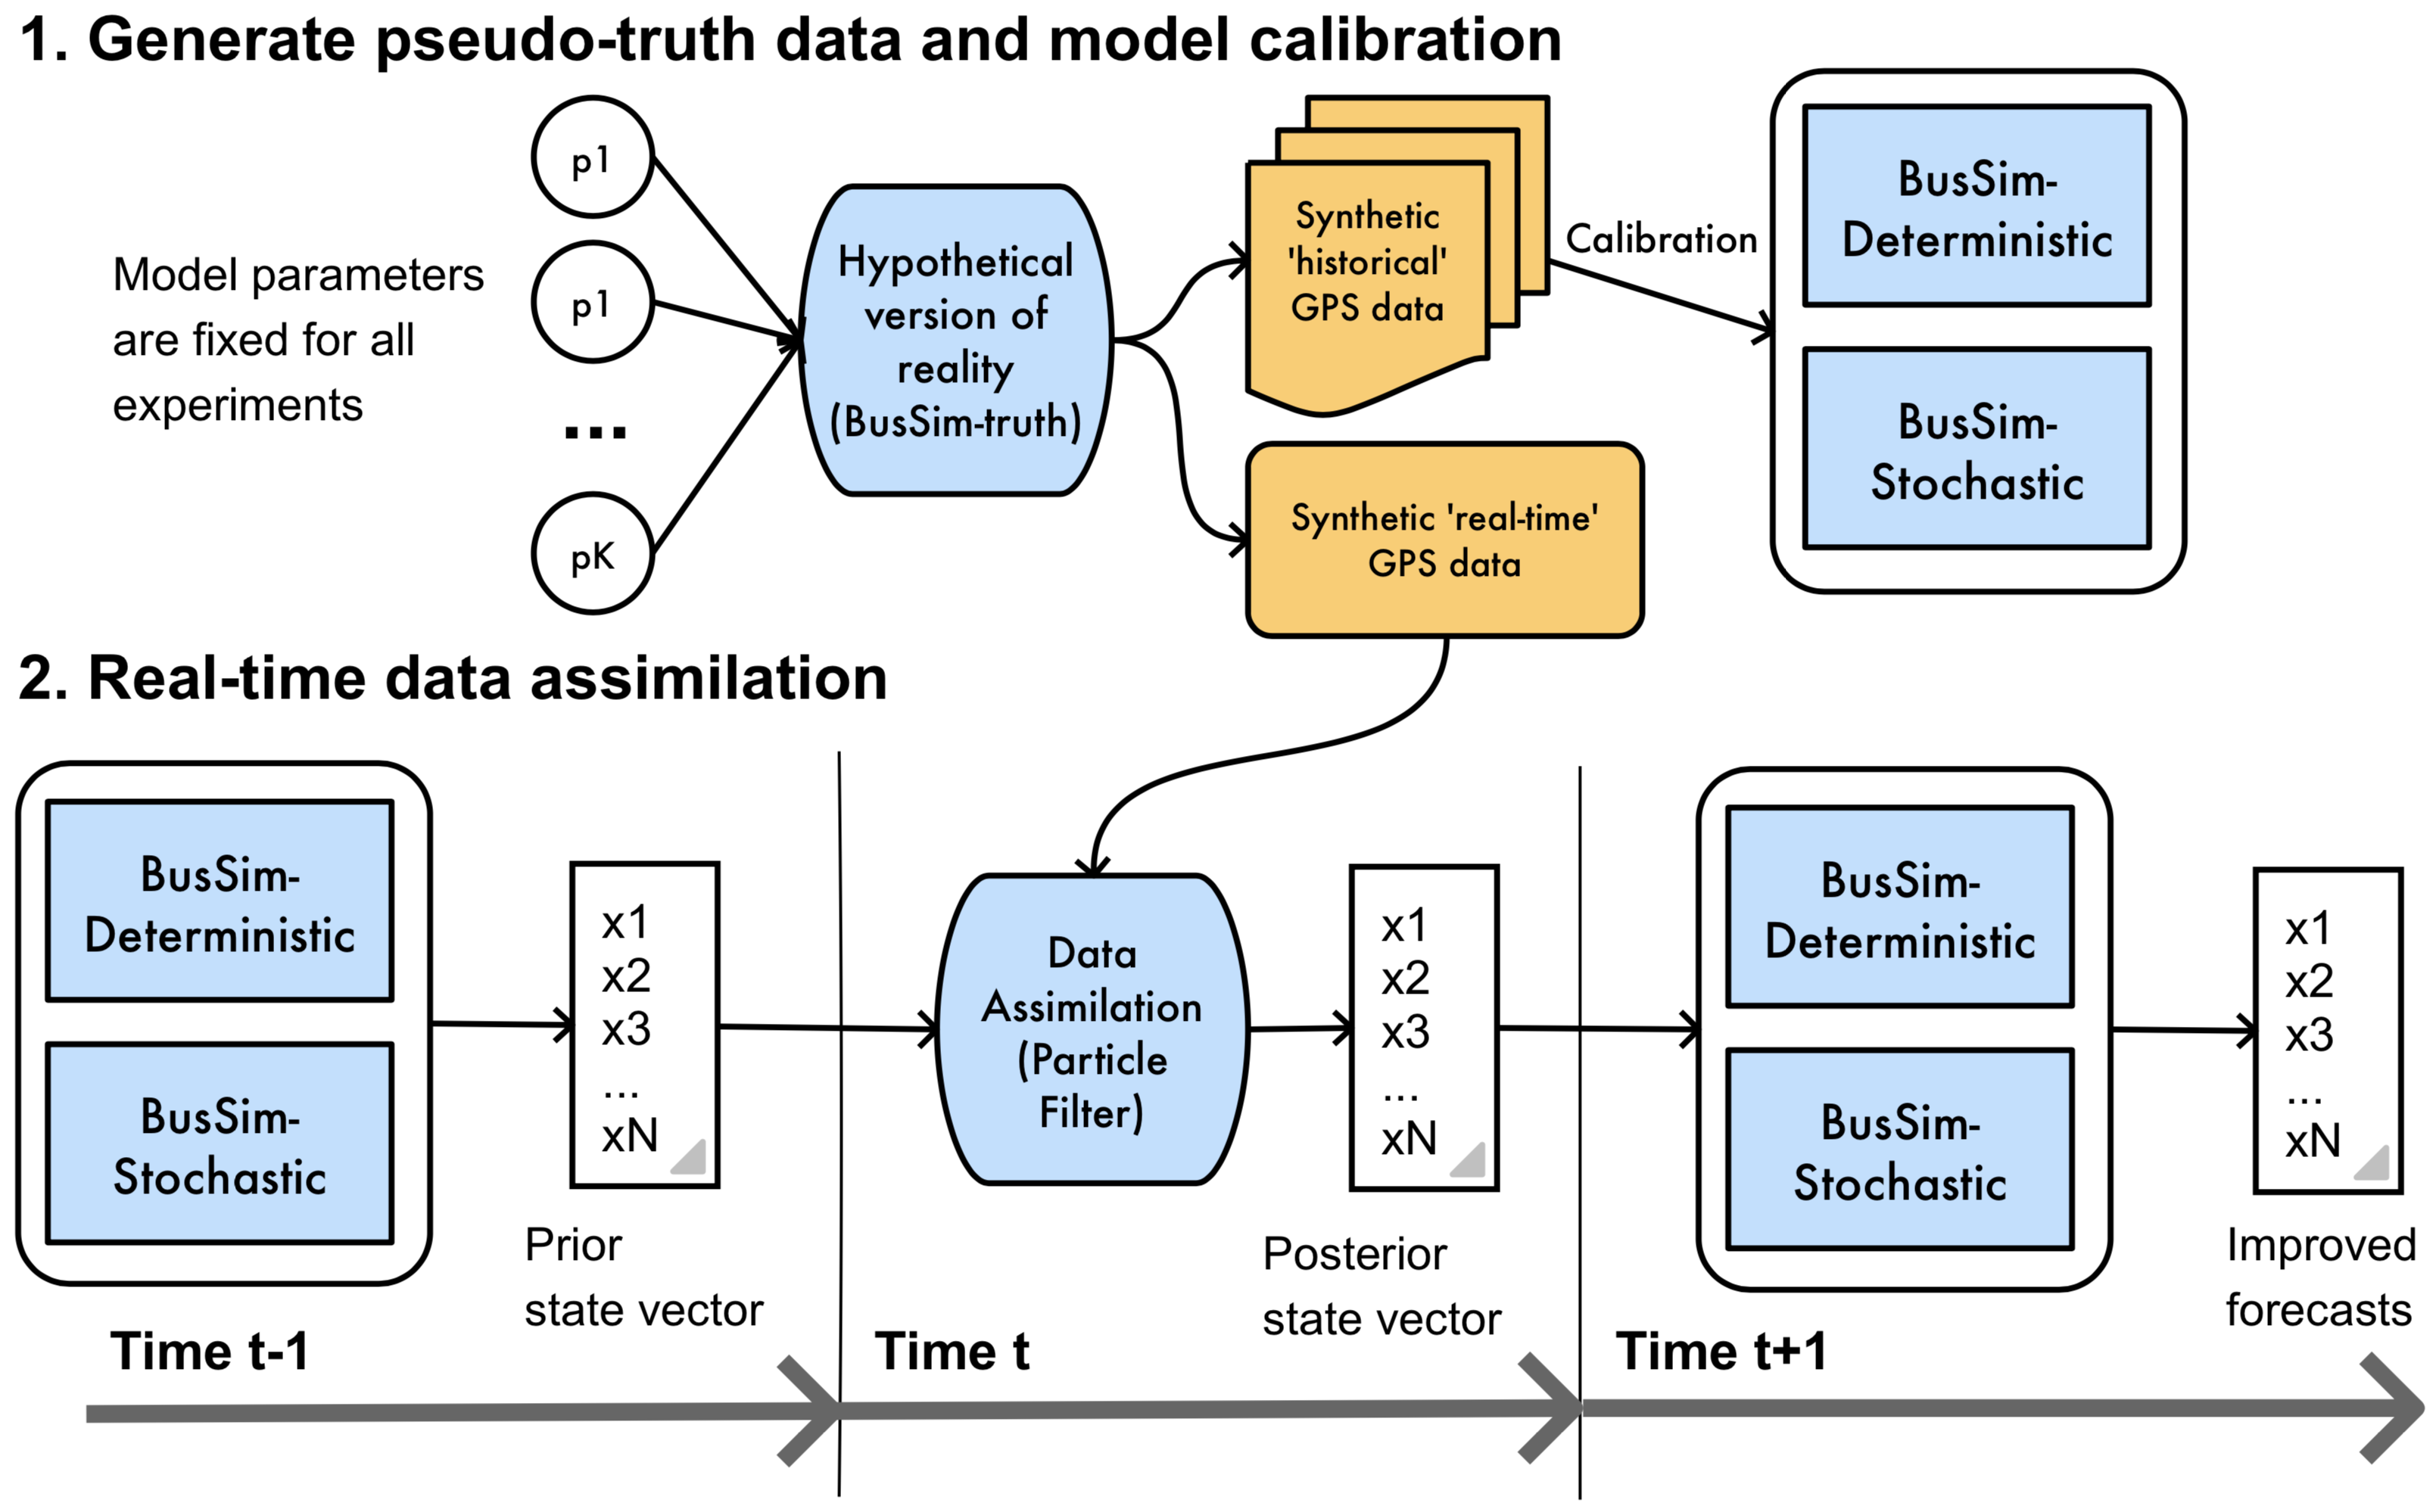
\includegraphics[width=13cm]{Figures/bussim-framework.png}
\caption{Study workflow.} 
\label{fig:workflow} 
\end{figure}

The study workflow generally consists of 2 major steps. It starts with the development of a Markovian ABM of bus route operation that will be referred as \textit{BusSim-truth}. BusSim-truth is a hypothetical version of reality and will be used to generate synthetic GPS data of bus locations with timestamps. Two sets of data will be generated. The first represents `historical' GPS data, which are essentially the outputs of multiple runs of the same BusSim-truth model with the same predefined set of parameters. The GPS data will be slightly different each time the model is run because BusSim-truth is stochastic (its outputs vary slightly from one run to another) and dynamic (the parameters that control factors such as the amount of traffic vary during a single model run). The second set of data represent a single run of BusSim-truth, also using the same set of parameters. These data will represent synthetic `real-time' GPS data and will be used to conduct data assimilation. This situation is similar to the reality, where `historical' data across multiple days are used to calibrate models and `real-time' data represent the \textit{current} state of the world. BusSim-truth will be reasonably realistic and will replicate popular phenomenon in bus operations such as bus bunching (two buses of the same line arrive at the same bus stop at the same time). 

In reality, any simulation model is a simplification of the actual dynamics. Taking this into consideration, we develop two simpler variations of BusSim-truth, knowing that they would not be able to perfectly represent the dynamics in BusSim-truth.  The two variations are: 
\begin{itemize} 
	\item \textbf{BusSim-deterministic}. This model evolves exactly the same way in each model run;
	\item \textbf{BusSim-stochastic}. This model is stochastic, e.g. the numbers of people waiting at bus stops is drawn from a random distribution 
\end{itemize} 

As would be necessary in reality, BusSim-deterministic and BusSim-stochastic will first be calibrated against the synthetic `historical' GPS data. In the second step of the study workflow, DA will be used in an attempt to update the states of the models to the `real-time' GPS observations in order to produce more accurate short-term forecasts of the system behaviour. 


% !TEX root = ParticleFilter.tex
\section{Method\label{Method}}

\begin{itemize}
\item Intro to station sim. Point to ODD
\item Intro to particle filter
\item Outline of experiments, including criteria to measure `success' of the PF
\end{itemize}

\subsection{The Agent-Based Model: StationSim}

XXXX outline stations sim


\subsection{Data Assimilation - Introduction and Definitions}

XXXX Outline how data assimilation method works broadly (e.g. \textit{update} and \textit{predict}) and define general concepts / objects.


\subsection{The Particle Filter}

Here, the \textit{state vector} contains all the information that a transition function needs to iterative the model forward by one step, including all of the agent ($i = \{ 0, 1, \dots, N \} $) parameters ($\overrightarrow{p_i}$) and variables ($\overrightarrow{v_i}$) as well as global model parameters $\overrightarrow{P}$:

\begin{equation}
  S  = \left[ \begin{array}{cccccccc}
\overrightarrow{p_0} & \overrightarrow{v_0} & \overrightarrow{p_1} &  \overrightarrow{v_1} &  \dots &  \overrightarrow{p_N} &  \overrightarrow{v_N} & \overrightarrow{P} 
\end{array} \right]
\end{equation} 

The \textit{observation vector} contains all of the observations made from the `real world' (in this case the pseudo-truth model) that the particle filter uses to predict the current true state, with the addition of some Gaussian noise, $\epsilon$:

\begin{equation}
  O  = \left[ \begin{array}{ccccccc}
x_0 & y_0 & x_1 & y_1 & \dots & x_n & y_n 
\end{array} \right]
\end{equation} 

In this paper, the particle filter is not used to estimate the state of the models variables ($\overrightarrow{v_i}$), not any of the parameters ($\overrightarrow{p_i}$ and \overrightarrow{P}) -- although it is worth noting that parameter estimation is technically feasible and will be experimented with in later iterations of this work. Therefore in the experiments conducted here, all parameters are fixed. Hence a further vector is required to map the observations to the state vector that the particle can actually manipulate. We define the partial state vector $S_\textrm{partial}$ to match the shape of $O$, i.e.:

\begin{equation}
  S_\textrm{partial}  = \left[ \begin{array}{ccccccc}
x_0 & y_0 & x_1 & y_1 & \dots & x_n & y_n 
\end{array} \right]
\end{equation} 





% !TEX root = ParticleFilter.tex
\section{Experiments\label{experiments}}

\subsection{Experiments with Uncertainty}

Purpose here is basically to see how the particle filter behaves when we give it l

\begin{enumerate}
\item Randomness in particles
\item Measurement noise (external)
\item Internal randomness (e.g. in agent behaviour)
\item (Simultaneous combinations of different randomness)
\end{enumerate}

\subsection{Experiments with Measurement Noise}

\begin{enumerate}
\item Reduce the amount of information given to the particle filter (e.g. only allow it to optimise half of the state vector).
\item Aggregate the measurements (e.g. counts per area rather than individual traces).
\end{enumerate}



% !TEX root = BusSim.tex
\section{Implications\label{s:implications}}

This paper presents an integrated framework to reduce uncertainty in ABMs when making predictions in real time, by combining parameter calibration and data assimilation. As discussed in Section \ref{s:Intro} and \ref{s:problem}, an `identical twin' approach has been adopted instead of real noisy data to facilitate an effective evaluation of the proposed methods against the synthetic `ground truth'. The numerical experiment shows that the framework yields more accurate predictions than (i) a benchmark scenario (without parameter calibration), and (ii) a scenario with parameter calibration but without data assimilation. 

In its current form, the framework can provide \textit{real time} bus locations and arrival times for passenger information systems. The forecasted bus location and arrival information provides key intelligence for waiting passengers \cite{fan2016waiting}. This is beneficial for all public transport passengers, but can be of particular benefit in countries, for example in the Global South \cite{kumar2017bus} where  there are frequent delays due to transport systems being complex, heterogeneous or heavily congested. The prediction of bus arrival times is also critical for real-time trip planners. These planning systems propose optimal alternative routes for passengers, or update information on a connecting service that may be unreachable due to delayed buses. 

Many advanced Intelligent Transport System applications heavily rely on predictions of bus location and arrival times, for  example  bus control studies such as \cite{daganzo2009headway}.  A model-based prediction of bus location and arrival time, such as the framework in this paper, would allow bus operators the ability to evaluate and update their transportation infrastructures in real time.



% !TEX root = BusSim.tex
\section{Conclusion\label{s:conclusion}}

This paper proposes parameter calibration and data assimilation frameworks to enhance the prediction accuracy in agent-based models (ABM) when the system under study has a \textit{stochastic} and \textit{dynamic} nature. This is done in a 'identical twin' approach. We first develop a stochastic and dynamic ABM of bus route, referred to as \textit{BusSim-truth}. This model is employed to generate synthetic `historical' and `real-time' GPS data of bus locations. The `historical' data is used to train two simpler models of bus route, referred to as \textit{BusSim-deterministic} and \textit{BusSim-stochastic}, and evaluate against the 'real-time' data. 

Similar to the practice, when any simulation model is a simplification of the reality, BusSim-deterministic and BusSim-stochastic are simpler than BusSim-truth, and thus may not be able to produce a prediction similar to the synthetic `real-time' GPS data under limited data. We propose a solution for this issue by parameter calibration using Cross-Entropy Method (Scenario 2), by a combination of parameter calibration and Particle Filtering (Scenario 3), and show that they outperform the no calibration scenario (Scenario 1) and only Particle Filtering scenario (Scenario 4), at various levels of uncertainty. 

This paper shows the need for parameter calibration and data assimilation, and particularly the combination of them, to improve the accuracy of model-based prediction using ABMs in real time. Future research direction includes fitting the proposed framework with real data instead of synthetic data. 

\section*{Data Availability} This paper does not use any real data. Synthetic data has been generated from one of its models (BusSim-truth model). The source code for all the models, and the used synthetic data are available from \url{https://github.com/leminhkieu/Bus-Simulation-model}. 

\section*{Competing interests} We declare we have no competing interests

\section*{Acknowledgements} This project has received funding from the
European Research Council (ERC) under the European Union Horizon 2020 research and innovation programme (grant agreement No. 757455), a UK Economic and Social Research Council (ESRC) Future Research Leaders grant (ES/L009900/1) and a ESRC/Alan Turing Joint Fellowship
(ES/R007918/1).

\appendix % !TEX root = BusSim.tex
\section*{Appendix A: The BusSim model \label{appendix:BusSim}}

Figure 2 illustrates the workflow for BusSim-truth. At each current time step $t$, each Bus agent checks whether the next time step would be larger than the vehicle's scheduled dispatch time $\delta_j$. If $t>\delta_j$, we then check whether the bus is on the road (Status equals $MOVING$), or at a stop for passenger dwelling (Status equals $DWELLING$), or has finished its service (Status equals $FINISHED$), otherwise the bus remains $IDLE$. 

If the status is $MOVING$, we first check whether the bus is at a bus stop, by comparing the $GeoFence$ area of each bus stop agent with the bus' location. If the bus is not approaching a bus stop, its current speed $v_j$ will be compared with the surrounding traffic speed $V$. If $v_j<V$, we assume that the bus will speed up with an acceleration rate $a_j$, thus we have: 
\begin{equation}
v_j^{t} = v_j^{t-dt} + a_j \cdot dt
\end{equation}

Therefore for the next time step, the bus will cover a distance of: 
\begin{equation}
S_j^t = S_j^{t-dt} + v_j^t \cdot dt
\end{equation}

If the speed already matches the traffic speed $V$, the bus will maintain the same speed. Or else if the bus is approaching a bus stop, the system will first check if the stop is the last stop. If it is the last stop, then the bus' status will be changed to $FINISHED$ and bus speed is changed to zero. If it is not the last stop, the system will change the status of agent Bus $j$ to $DWELLING$ and its speed to zero. The number of boarding and alighting passengers from the bus $j$, and the time that it will leave the stop are estimated as follows.  

The number of boarding passenger is proportional to the time gap between the current time (when Bus $j$ approaches the bus stop $m$) and the last time any bus visits the bus stop $m$:     
\begin{equation}
B_{j,m} = \nint{Po(Arr_m \cdot (t^a_{j+1,m}-t^a_{j,m}) } \quad | \quad B_{j,m}\in\mathbb{N}
\label{eq:Boarding_est}
\end{equation}

Equation \ref{eq:Boarding_est} shows that the number of boarding passengers is estimated using a stochastic Poisson process. A Poisson process is widely adopted in literature to estimate the count of passengers waiting at a public transport stop \citep{toledo2010mesoscopic,cats2010mesoscopic}. Extensions of this stochastic process have been introduced, such as non-homogeneous Poisson process \citep{kieu2018stochastic}, where the arrival rate is time-dependent, but for simplicity we adopt a homogeneous Poisson process for this paper. Equation \ref{eq:Boarding_est} makes the BusSim-truth model stochastic, because there is randomness in the way the Poisson process generates a number. For more details on the number generation process using stochastic Poisson process (e.g. thinning algorithm), interested readers may refer to \citep{lewis1979simulation}. The number of boarding passengers is also limited by the available capacity of the bus:
\begin{equation}
B_{j,m} = \text{max} \big( B_{j,m}, C - Occ_m )   \big)
\label{eq:Boarding_limit}
\end{equation}

The number of alighting passengers is proportional to the number of passenger on board (bus occupancy) and the departure rate at the stop $m$.  For simplicity, we assume that $A_{j,m}$ is the product between the departure rate from bus stop $m$ and the current bus occupancy (the number of passenger on board leaving the last stop): 
\begin{equation}
A_{j,m} = \nint{Dep_m \cdot Occ_{j,m-1}} \quad | \quad A_{j,m}\in\mathbb{N}
\end{equation}

To estimate the amount of time that bus will have to stay at the bus stop $m$ for passenger boarding and alighting, a.k.a. \textit{dwell time} $D_{j,m}$, we adopt the approach in \citep{bertini2004modeling} and the Transit Capacity and Quality of Service Manual (TCQSM) \citep{kfh2013transit}:
\begin{equation}
D_{j,m} = \theta_1 + \theta_2 \times B_{j,m} + \theta_3 \times A_{j,m} 
\label{eq:dwell_time}
\end{equation}
The parameter set [$\theta_1,\theta_2,\theta_3$] represents the time spent for passenger boarding, alighting, and a fixed value for vehicle stopping and starting, respectively. Equation \ref{eq:dwell_time} is the formulation for a single-door bus system, where boarding and alighting occurs sequentially. 

The departure time of bus $j$ from stop $m$ is calculated from the arrival time $t^a_{j,m}$ plus the time spent at stops for passenger boarding and alighting, or in other words the dwell time $D_m$:
\begin{equation}
t^d_{j,m} = t^a_{j,m} + D_{j,m}
\end{equation}
In BusSim, the bus $j$ is only allowed to leave the bus $m$ at time $t^d_{j,m}$, so this is also called the $Leave\_stop\_time$, as can be seen in the Figure 2. 

If the status of bus $j$ is $DWELLING$, it is at a stop for passenger boarding and alighting. We then check if the next time step would be larger or equal to the leave stop time $t^d_{j,m}$. If it would, then the bus would start accelerate to leave the stop, otherwise it would stay for at least another time interval. Finally, if the status of the bus is $FINISHED$, then we would do nothing. The modelling process then moves to the next Bus agent until the last Bus, then the whole model moves to the next time step until the last time step. 

BusSim-truth also assumes that parameters dynamically change over time by introducing an additional parameter $\xi$ to represent the change in passenger demand or surrounding traffic speed. For simplicity, we assume that a single, deterministic parameter $\xi$ can model these dynamic changes. In practice, it is possible, and more desirable, to use a time-dependent value of $\xi$ such that dynamic change is better captured, and multiple $\xi$ to model different changes. $\xi>0$ represents an increase in passenger demand and traffic speed, and $\xi<0$ represents otherwise. In this paper, the change in passenger demand or traffic speed is modelled as: 
\begin{align}
V = V \cdot \big( 1 - \frac{t}{T} \cdot \frac{100}{\xi} \big) \\
Arr_m = Arr_m \cdot (1 - \frac{t}{T} \cdot \frac{100}{\xi}
\label{eq:dynamic_bussim}
\end{align}
A positive value of $\xi$ in Equation \ref{eq:dynamic_bussim} gradually reduces the surrounding traffic speed $V$ and increases the arrival rate $Arr_m$, which would lead to more bus delays and congestion. 

\appendix \section*{Appendix B: Cross Entropy Method for Parameter Calibration}

This Appendix describes the pseudocode for the Cross Entropy Method for Normal distribution \citep{rubinstein1999cross}. 

\begin{algorithm} [H]	
	%\scriptsize
	\SetAlgoLined
	Set $p=(\mu_1,\sigma_1,\mu_2,\sigma_2,...,\mu_K,\sigma_K)$ \quad \%Initial distribution parameters 
	
	Set $M$ \quad     \%Number of stops
	
	Set $T$  \quad  \% Maximum iteration number
	
	Set $I$  \quad  \% Maximum iteration number 
	
	Set $\rho$  \quad \% Set selection ratio
	
	\For {$t$ from 1 to $T$} { \  \%Main CEM loop
	
	    \For {$i$ from 1 to $I$} {
	
	Draw $y^{(i)}$ from $\mathcal{N}(\mu,\sigma)$  \quad  \%Draw $I$ samples
	
	Compute $f^i:=f(y^{(i)}$}
	
	Sort $f^i$-values \quad  \%Order by decreasing magnitude
	
	$\gamma \leftarrow f_{\rho.I}$ \quad  \%Set threshold 
	
	$L_\gamma \leftarrow \{ y^{(i)} | f(y^{(i)}) \leq \gamma$  \quad  \%Collect elite samples 
	
	$\mu'_j = \frac{1}{L_\gamma} \sum_{i=1}^{L_\gamma} \mu_{i,j}$  \quad  \%Update $\mu$

	$\sigma'_j = \frac{1}{L_\gamma} \sum_{i=1}^{L_\gamma} \sigma_{i,j}$   \quad  \%Update $\sigma$
	
	$\mu_j \leftarrow \alpha \mu'_j + (1 - \alpha)  \mu_j$ \quad \%Update with step size $\alpha$
	
	$\sigma_j \leftarrow \alpha \sigma'_j + (1 - \alpha)  \sigma_j$ \quad \%Update with step size $\alpha$
	}
	\caption{Cross-Entropy Method for Normal distribution}
	\label{algo:CEM}
\end{algorithm}

%\section*{References}

\bibliographystyle{plain} 
\bibliography{2018-pf-bussim}

\end{document}